%% LyX 2.3.4.2 created this file.  For more info, see http://www.lyx.org/.
%% Do not edit unless you really know what you are doing.
\documentclass[english]{article}
\usepackage[T1]{fontenc}
\usepackage[latin9]{luainputenc}
\usepackage[a4paper]{geometry}
\geometry{verbose,tmargin=2cm,bmargin=2cm,lmargin=2cm,rmargin=2cm}
\usepackage{amsmath}
\usepackage{graphicx}
\usepackage{babel}
\begin{document}
\title{\textbf{Notes on DDA0.1}}
\author{Augustin Muster}

\maketitle
\tableofcontents{}

\section{DDA method description}

\subsection{Lattice and polarisabilities}

Let us consider a solid of volume $V$ discretized in $N$ dipoles
on a cubic lattice (of lattice parameter $d$) with dielectric tensor
$\varepsilon(\boldsymbol{r})$ in a homogoneous medium with dielectric
constant $\varepsilon_{h}$such that
\begin{equation}
V=Nd{{}^3}.
\end{equation}
Each dipole is associated with his position $\boldsymbol{r_{n}}$,
$n=1,...,N$and his quaisitatic polarisability tensor defined by
\begin{equation}
\boldsymbol{\alpha}_{n0}=(\epsilon(\boldsymbol{r_{n}})-\epsilon_{h}I)((\epsilon(\boldsymbol{r_{n}})-\epsilon_{h}I)+\boldsymbol{L_{n}^{-1}}\epsilon_{h})^{-1}\boldsymbol{L_{n}^{-1}}V_{n},\label{eq:quasis}
\end{equation}
where $\boldsymbol{I}$ \textasciicircum is the identy matrix, $V_{n}=d{{}^3}$
is the volume of a discretization unit and $\boldsymbol{L_{n}}$is
the depolarisation tensor defined as
\begin{equation}
[\boldsymbol{L}_{n}]_{ij}=\delta_{ij}\frac{1}{3}\label{eq:depol}
\end{equation}
for a cube. A radiative correction of the polarisability has to be
taken into account. With this correction, the polarisability tensor
$\boldsymbol{\alpha}_{n}$ now reads7
\begin{equation}
\boldsymbol{\alpha}_{n}=\left(\boldsymbol{\alpha}_{n0}^{-1}-i\frac{k{{}^3}}{6\pi}\right)^{-1},\label{eq:radiative}
\end{equation}
where $k$ is the wavenumber of the incident wave.

\subsection{Scattering}

Let us consider that the solid is illuminated by an inciedent field
$\boldsymbol{E}_{0}(\boldsymbol{r})$ the field $\boldsymbol{E}_{exc}(\boldsymbol{r}_{n})$
extiting the nth dipole is equal to the incident field plus the contribution
of the other dipoles, i.e. 

\begin{equation}
\boldsymbol{E}_{exc}(\boldsymbol{r}_{n})=\boldsymbol{E}_{0}(\boldsymbol{r}_{n})+k{{}^2}\sum_{m\neq n}^{N}\boldsymbol{G}(\boldsymbol{r}_{n},\boldsymbol{r}_{m})\boldsymbol{\alpha}_{m}\boldsymbol{E}_{exc}(\boldsymbol{r}_{m}),
\end{equation}
where $\boldsymbol{G}(\boldsymbol{r}_{n},\boldsymbol{r}_{m})$ is
the green tensor which reads

\begin{equation}
\boldsymbol{G}(\boldsymbol{r}_{n},\boldsymbol{r}_{m})=\frac{\exp(ikR)}{4\pi R}\left(\left(1+\frac{i}{kR}-\frac{1}{k{{}^2}R{{}^2}}\right)\boldsymbol{I}-\left(1+\frac{3i}{kR}-\frac{3}{k{{}^2}R{{}^2}}\right)\frac{\boldsymbol{R}\otimes\boldsymbol{R}}{R{{}^2}}\right),\label{eq:Gtensor}
\end{equation}
with $\boldsymbol{R}=\boldsymbol{r}_{n}-\boldsymbol{r}_{m}$, $R=|\boldsymbol{R}|$.
This equation in then just a big system of 3N linear equations that
reads 

\begin{equation}
\begin{bmatrix}\boldsymbol{I} & \dots & -k{{}^2}\boldsymbol{G}(\boldsymbol{r}_{1},\boldsymbol{r}_{N})\boldsymbol{\alpha}\\
\vdots & \ddots & \vdots\\
-k{{}^2}\boldsymbol{G}(\boldsymbol{r}_{N},\boldsymbol{r}_{1})1 & \dots & \boldsymbol{I}
\end{bmatrix}\left[\begin{array}{c}
\boldsymbol{E}_{exc}(\boldsymbol{r}_{1})\\
\vdots\\
\boldsymbol{E}_{exc}(\boldsymbol{r}_{N})
\end{array}\right]=\left[\begin{array}{c}
\boldsymbol{E}_{0}(\boldsymbol{r}_{1})\\
\vdots\\
\boldsymbol{E}_{0}(\boldsymbol{r}_{N})
\end{array}\right]\label{eq:DDAeq}
\end{equation}
that can be solved in order to get the $\boldsymbol{E}_{exc}(\boldsymbol{r}_{n})$.
Using this, the polarizations of each dipole can be computed using
$\boldsymbol{P}_{n}=\boldsymbol{\alpha}_{n}\boldsymbol{E}_{exc}(\boldsymbol{r}_{n})$

\subsection{Cross sections calculations}

Then, the extinction, absorbtion and scattering cross section $\sigma_{ext},\sigma_{abs},\sigma_{sca}$
(that follows $\sigma_{ext}=\sigma_{abs}+\sigma_{sca}$) can be comuted
using (considerning that the incident field is a plane wave $\boldsymbol{E}_{0}(\boldsymbol{r})=\boldsymbol{E}_{0}\exp(ikr)$))

\begin{equation}
\sigma_{ext}=\frac{k}{\epsilon_{h}|\boldsymbol{E}_{o}|{{}^2}}\sum_{n=1}^{N}Im(\boldsymbol{E}_{0}^{*}(\boldsymbol{r})\cdot\boldsymbol{P}_{n})
\end{equation}
\begin{equation}
\sigma_{sca}=\frac{k{{}^3}}{\epsilon_{h}{{}^2}|\boldsymbol{E}_{o}|{{}^2}}\sum_{n,m=1}^{N}\boldsymbol{P}_{n}^{*}\cdot Im(\boldsymbol{G}(\boldsymbol{r}_{n},\boldsymbol{r}_{m}))\boldsymbol{P}_{n}
\end{equation}
\begin{equation}
\sigma_{abs}=\frac{k}{\epsilon_{h}{{}^2}|\boldsymbol{E}_{o}|{{}^2}}\sum_{n=1}^{N}Im(\boldsymbol{P}_{n}\cdot(\boldsymbol{\alpha}_{n0}\boldsymbol{P}_{n})^{*})
\end{equation}


\section{DDA0.1 documentation}

The code is divided in several modules that can be easily inculded
in other modules and easily extended. The core functionalities of
the DDA are in impolemented in the \textbf{DDA.jl. }This code as well
as all the others module providing side- but essential functionalities
are describet in this section.

\subsection{DDA.jl}

DDA.jl contains the core functionalyty of the DDA, i.e. the functions
to compute the green tensor and solve the linear system of equations.
These functions are availeble either in a normal or ``dimensionless''
version. They are the following.

\subsubsection{solve\_DDA()}

\textbf{solve\_DDA(knorm, r, alpha, input\_field::Function ; output=\textquotedbl polarisations\textquotedbl ,
solver=\textquotedbl LU\textquotedbl , verbose=true)}

This function generate the DDA equations systems (equation (\ref{eq:DDAeq}))
and solve it in order to output the polarisations $\boldsymbol{P}_{n}$or
the inverse of the linear equation matrix $A^{-1}$.

\paragraph{Arguments}
\begin{itemize}
\item \textbf{knorm: }norm of the k vector (real scalar).
\item \textbf{r: }real array containing all the (3d) position vectors of
the dipoles.
\item \textbf{alpha: }complex array containing all the (3x3) polarisability
tensor of each dipole.
\item \textbf{input\_field: }pointer to a function that will generate the
input field this function haa.
\item \textbf{output }(facultative): it can takes two values: ``polaristions''
(the function returns the $\boldsymbol{P}_{n}$) or ``matrix'' (the
functiuons return the $A^{-1}$). By default set to ``polarisations''.
\item \textbf{solver }(facultative): indication on which solver to use to
solve the equations. There is yet only one possibility: ``LU'' (use
the LU decomposition of LAPACK).
\item \textbf{verbose }(facultative): whether to print everything or not.
By default set to ``true''.
\end{itemize}

\paragraph{Outputs}

An array of size (N,3) with the polarisations $\boldsymbol{P}_{n}$
or the inverse of the (3N{*}3N) linear equation matrix $A^{-1}$ (dependint
on the \textbf{output }parameter).

\subsubsection{green()}

\textbf{green(r1, r2, knorm)}

This function computes the green tensor using equation (\ref{eq:Gtensor}).

\paragraph{Arguments}
\begin{itemize}
\item \textbf{r1: }position of the first dipole (3d vector)
\item \textbf{r2: }position of the first dipole (3d vector)
\item \textbf{knorm: }norm of the k vector
\end{itemize}

\paragraph{Outputs}

The associated (3x3) green tensor.

\subsubsection{solve\_DDA\_dl()}

\textbf{solve\_DDA\_dl(knorm, kr, k3alpha, input\_field::Function
; output=\textquotedbl polarisations\textquotedbl , solver=\textquotedbl LU\textquotedbl ,
verbose=true)}

This function generate the DDA equations systems (equation (7)) with
dimensionless inputs and solve it in order to output the polarisations
$\boldsymbol{P}_{n}$or the inverse of the linear equation matrix
$A^{-1}$.

\paragraph{Arguments}
\begin{itemize}
\item \textbf{knorm: }norm of the k vector (real scalar).
\item \textbf{kr: }real array containing all the (3d) position vectors of
the dipoles, multiplied with the norm of the k vector
\item \textbf{k3alpha: }complex array containing all the (3x3) polarisability
tensor of each dipole multiplied with norm of the k vector to the
power 3.
\item \textbf{input\_field: }pointer to a function that will generate the
input field this function haa.
\item \textbf{output }(facultative): it can takes two values: ``polaristions''
(the function returns the $\boldsymbol{P}_{n}$) or ``matrix'' (the
functiuons return the $A^{-1}$). By default set to ``polarisations''.
\item \textbf{solver }(facultative): indication on which solver to use to
solve the equations. There is yet only one possibility: ``LU'' (use
the LU decomposition of LAPACK).
\item \textbf{verbose }(facultative): whether to print everything or not.
By default set to ``true''.
\end{itemize}

\paragraph{Outputs}

An array of size (N,3) with the polarisations $\boldsymbol{P}_{n}$
or the inverse of the (3N{*}3N) linear equation matrix $A^{-1}$ (dependint
on the \textbf{output }parameter).

\subsubsection{green\_dl()}

\textbf{green\_dl(kr1, kr2, knorm)}

This function computes the green tensor with dimensionless inputs
using equation (6).

\paragraph{Arguments}
\begin{itemize}
\item \textbf{kr1: }position of the first dipole times the norm of the wave
vector (3d vector)
\item \textbf{kr2: }position of the first dipole times the norm of the wave
vector (3d vector)
\item \textbf{knorm: }norm of the k vector (real scalar)
\end{itemize}

\paragraph{Outputs}

The associated (3x3) green tensor.

\subsection{alpha.jl}

The alpha.jl module is a side-functionality module providing functions
to compute the polarisability tensors.

\subsubsection{depolarisation\_tensor()}

\textbf{depolarisation\_tensor(lx,ly,lz,Vn)}

This function computes the depolarisation tensor as in equation (\ref{eq:depol})
but for an arbitrary parralelipipedic unit.

\paragraph{Arguments}
\begin{itemize}
\item \textbf{lx, ly, lz}: dimensions of the parralelipipedic volume (scalars).
\item \textbf{Vn: }volume of the parralelipipedic unit (scalar).
\end{itemize}

\paragraph{Outputs}

The (3x3) depolarisation tensor

\subsubsection{alpha\_0()}

\textbf{alpha\_0(e,e\_m,Ln,Vn)}

This function compute the quasistatic polarisability tensor as in
equation (\ref{eq:quasis}).

\paragraph{Arguments}
\begin{itemize}
\item \textbf{e: }dielectric permetivitty of the medium (complex scalar).
\item \textbf{e\_m: }dielectric permittivity of the embeding medium (complex
scalar).
\item \textbf{Ln: }depolaristion tensor (3x3 matrix).
\item \textbf{Vn: }volume of the particle (scalar)
\end{itemize}

\paragraph{Outputs}

The associated (3x3 complex) quasistatic polarisability tensor.

\subsubsection{alpha\_radiative()}

\textbf{alpha\_radiative(a0,knorm)}

This function compute the polarisability tensor with the radiative
correction with equation (\ref{eq:radiative}), given a quasitatic
polarisability tensor.

\paragraph{Arguments}
\begin{itemize}
\item \textbf{a0: }a quasistatic polarisability tensor (3x3 complex)
\item \textbf{knorm: }the norm of the k vector (scalar)
\end{itemize}

\paragraph{Outputs}

The (3x3 complex) polarisability tensor with radisative correction.

\subsection{input\_fields.jl}

The input\_fields.jl module is a side-functionality module providing
functions to generate the input fields.

\subsubsection{plane\_wave()}

\textbf{plane\_wave(knorm,r,khat={[}0,0,1{]},e0={[}1,0,0{]})}

Function to evaluate a plane wave at a given position.

\paragraph{Arguments}
\begin{itemize}
\item \textbf{knorm: }the norm of the k vector (scalar).
\item \textbf{r: }position where to evaluate the plane wave (3d vector).
\item \textbf{khat }(faculatitve): direction of the k vector (3d vector).
The norm of this vector must be 1. By default set to the direction
of the plane wave.
\item \textbf{e0 }(facultative): polarisation (3d complex vector). By default
set to {[}1,0,0{]} (polarized on the x axis).
\end{itemize}

\paragraph{Outputs}

A 3d complex vector representing the plane wave vector at the given
position.

\subsubsection{plane\_wave\_dl()}

\textbf{plane\_wave\_dl(kr,khat={[}0,0,1{]},e0={[}1,0,0{]})}

Function to evaluate a plane wave at a given position, but with dimensionless
inputs.

\paragraph{Arguments}
\begin{itemize}
\item \textbf{kr: }position where to evaluate the plane wave times the norm
of the k vector (3d vector).
\item \textbf{khat }(faculatitve): direction of the k vector (3d vector).
The norm of this vector must be 1. By default set to the direction
of the plane wave.
\item \textbf{e0 }(facultative): polarisation (3d complex vector). By default
set to {[}1,0,0{]} (polarized on the x axis).
\end{itemize}

\paragraph{Outputs}

A 3d complex vector representing the plane wave vector at the given
position.

\subsection{processing.jl}

\subsubsection{compute\_cross\_sections()}

\textbf{compute\_cross\_sections(knorm,p,e\_inc,alpha0,r;e0={[}1,0,0{]},explicit\_scattering=true,verbose=true)}

Compute the extinction, absorbtion and scattering cross sections as
done in equations (8), (9) and (10) (only for a plane wave illumination!). 

\paragraph{Arguments}
\begin{itemize}
\item \textbf{knorm: }the norm of the k vector (scalar).
\item \textbf{p: }polarisations (array of 3d complex vectors).
\item \textbf{alpha0 }(facultative): quasistatic polarisability tensors
(array of complex 3x3 matrices).
\item \textbf{r: }real array containing all the (3d) position vectors of
the dipoles.
\item \textbf{e0 }(facultative): polarisation (3d complex vector). By default
set to {[}1,0,0{]} (polarized on the x axis).
\item \textbf{explicit\_scattering }(facultative): wether to compute the
scattering cross section explicitely or not. Bay default set to true.
\item \textbf{verbose }(facultative): whether to print everything or not.
By default set to ``true''.
\end{itemize}

\paragraph{Outputs}

an array containing {[}lambda,Cext, Cabs,Csca{]}

\section{Test and Example.}

DDA computations have been made with a silicon sphere with radius
of 230nm, with 13000 dipoles, $\lambda=1000,...,2000$nm. The script
used to run these computation is called \textbf{run\_DDA.jl}

\begin{figure}
\begin{centering}
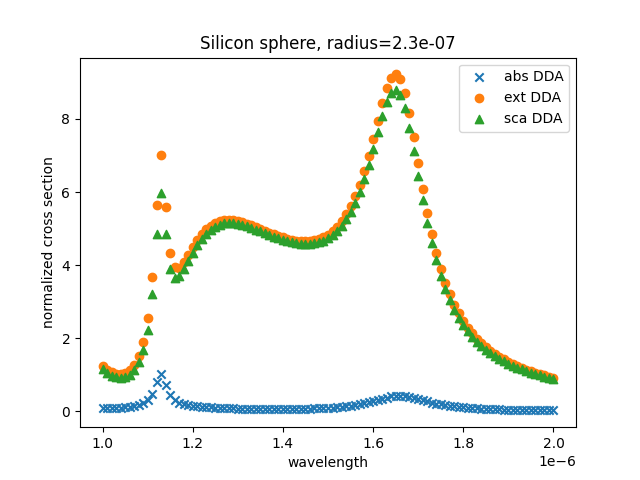
\includegraphics[width=12cm]{../../DDA/DDA0.1/notes/Silicon_cross_section_13000}\caption{Extinction,scattering and absorbtion cross sections for a silicon
sphere with radius of 230nm, computed with the DDA.jl code}
\par\end{centering}
\end{figure}
\begin{figure}
\centering{}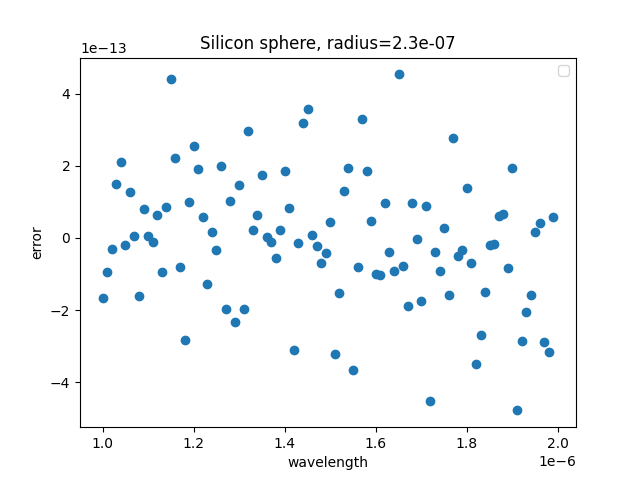
\includegraphics[width=12cm]{../../DDA/DDA0.1/notes/Silicon_cross_section_4100}\caption{relative error of the extinction for the computation of figure 1.}
\end{figure}
\begin{figure}
\centering{}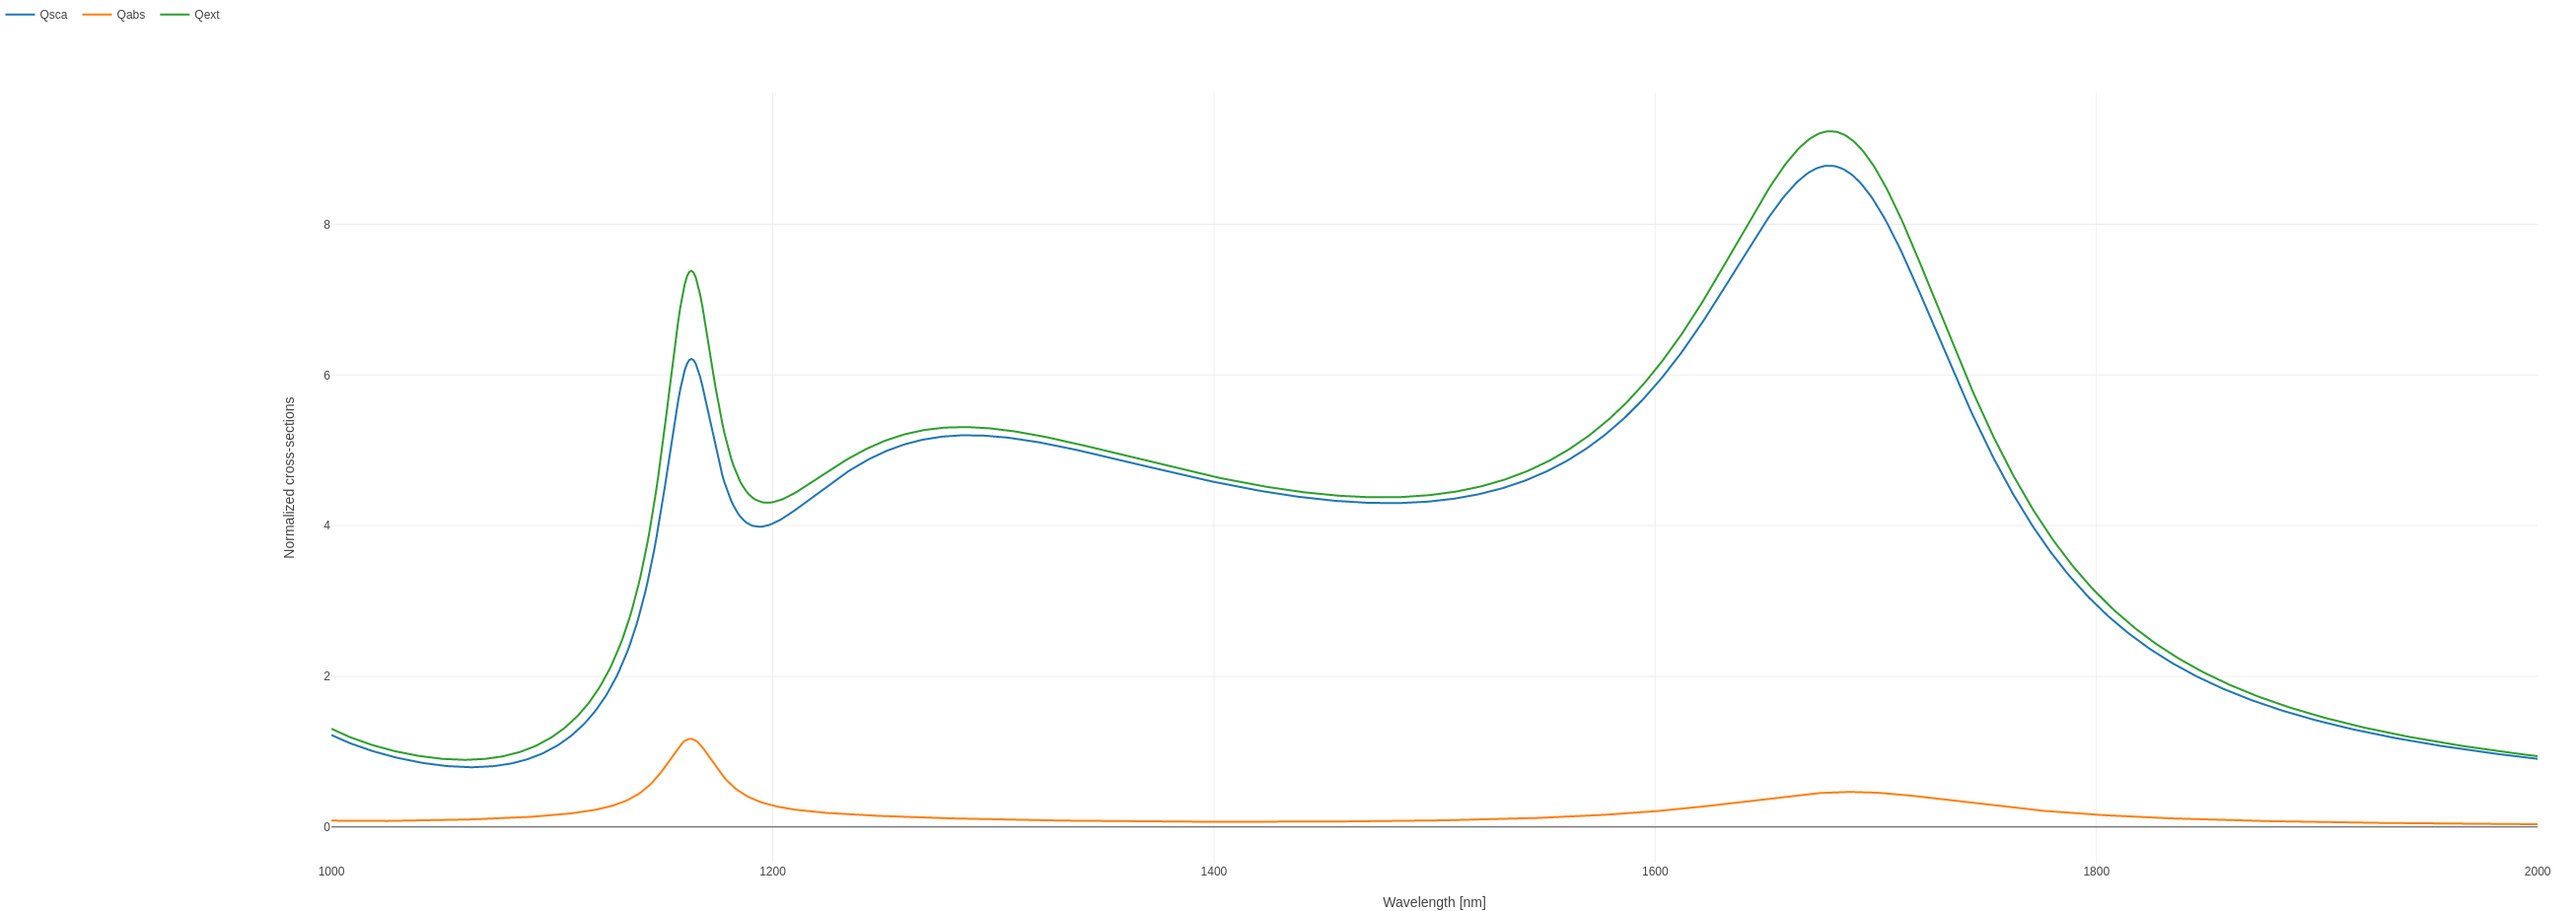
\includegraphics[width=15cm]{../../DDA/DDA0.1/notes/mieplot}\caption{Extinction,scattering and absorbtion cross sections for a silicon
sphere with radius of 230nm, computed with Mie theory}
\end{figure}

\end{document}
